\documentclass{standalone}
\usepackage{pgfgantt}
\usepackage{xcolor}
\usepackage{tikz}
\usepackage[normalem]{ulem}  % for strikethrough text
\usetikzlibrary{patterns,decorations.pathmorphing,shapes.geometric}

% Define a modern color palette
\definecolor{primaryblue}{RGB}{41,128,185}
\definecolor{secondaryblue}{RGB}{52,152,219}
\definecolor{lightblue}{RGB}{174,214,241}
\definecolor{accentgreen}{RGB}{39,174,96}
\definecolor{accentorange}{RGB}{230,126,34}
\definecolor{accentred}{RGB}{231,76,60}
\definecolor{darkgray}{RGB}{52,73,94}
\definecolor{lightgray}{RGB}{236,240,241}
\definecolor{mediumgray}{RGB}{149,165,166}
\definecolor{discardedgray}{RGB}{120,120,120}

% Legacy colors for compatibility
\definecolor{barblue}{RGB}{174,214,241}
\definecolor{groupblue}{RGB}{41,128,185}
\definecolor{linkred}{RGB}{231,76,60}

\newcounter{myWeekNum}
\stepcounter{myWeekNum}
\newcommand{\myWeek}{\themyWeekNum
    \stepcounter{myWeekNum}
    \ifnum\themyWeekNum=53
    \setcounter{myWeekNum}{1}
    \else\fi
}

\setganttlinklabel{s-s}{START-TO-START}
\setganttlinklabel{f-s}{FINISH-TO-START}
\setganttlinklabel{f-f}{FINISH-TO-FINISH}

\begin{document}
\setcounter{myWeekNum}{12}
\ganttset{%
    calendar week text={\myWeek{}},
    calendar month rule/.style={draw=black, thick} % style for vertical month lines
}

\begin{ganttchart}[
    time slot format=isodate,
    calendar week text={\myWeek{}},
    x unit=5pt,  % Slightly wider for better readability
    y unit title=0.6cm,
    y unit chart=0.8cm,
    % Enhanced canvas with subtle gradient effect
    canvas/.append style={fill=lightgray!20, draw=darkgray!30, line width=.5pt},
    % Sophisticated grid styling
    hgrid style/.style={draw=mediumgray!40, line width=.3pt},
    vgrid={*1{draw=mediumgray!30, line width=.2pt}},
    % Enhanced today marker
    today=2025-07-01,
    today rule/.style={
      draw=accentred,
      dash pattern=on 4pt off 3pt,
      line width=2pt,
      opacity=0.8
    },
    % Professional typography
    title/.append style={draw=none, fill=darkgray!10},
    title label font=\bfseries\large\color{darkgray},
    title height=1,
    % Enhanced bar styling with gradients and shadows
    bar label font=\bfseries\normalsize\color{darkgray},
    bar label node/.append style={left=3.2cm, align=left}, % Adjusted for longer text
    bar/.append style={
      draw=primaryblue!80,
      fill=primaryblue!70,
      line width=0.8pt,
      rounded corners=2pt
    },
    bar incomplete/.append style={
      fill=lightblue!60,
      draw=secondaryblue!60
    },
    bar progress label font=\footnotesize\color{white},
    bar progress label node/.append style={text=white},
    % Enhanced group styling
    group label font=\bfseries\Large\color{primaryblue},
    group label node/.append style={align=left},
    group progress label font=\bfseries\normalsize\color{primaryblue},
    group/.append style={
      draw=primaryblue!80,
      fill=primaryblue!20,
      line width=1.2pt,
      rounded corners=1pt
    },
    group peaks height=.6,
    group peaks width=.2,
    group peaks tip position=.5,
    % Enhanced milestone styling
    milestone label font=\bfseries\normalsize\color{accentred},
    milestone label node/.append style={left=3.2cm, align=left}, % Adjusted for longer text
    milestone/.append style={
      fill=accentred,
      draw=accentred!80,
      line width=1pt,
      shape=diamond
    },
    milestone height=0.6,
    % Month rule styling
    calendar month rule/.append style={draw=darkgray, line width=1.5pt}
  ]{2025-03-20}{2025-07-04}
  \gantttitlecalendar{month=name, week}\\

  \ganttgroup{Jan}{2025-03-22}{2025-07-04} \\
  \ganttbar[progress=100, bar/.append style={fill=accentgreen!70, draw=accentgreen!80}]{Repo Setup}{2025-03-22}{2025-03-28} \\
  \ganttbar[progress=100, bar/.append style={fill=accentorange!70, draw=accentorange!80}]{Explore Gemini SDK \& Image Understanding Notebooks}{2025-03-23}{2025-03-27} \\
  \ganttbar[progress=100, bar/.append style={fill=accentorange!60, draw=accentorange!70}]{Lit. Review (SpatialBot \( \rightarrow \) Video-3D LLM \( \rightarrow \) SpatialVLM + VQASynth)}{2025-03-31}{2025-04-01}
  \ganttbar[progress=100, bar/.append style={fill=accentorange!60, draw=accentorange!70}]{}{2025-04-19}{2025-04-25} \\
  \ganttbar[progress=100, bar/.append style={fill=primaryblue!70, draw=primaryblue!80}]{Stray Scanner Parser \& Dataset}{2025-04-01}{2025-04-04} \\
  \ganttbar[progress=100, bar/.append style={fill=secondaryblue!70, draw=secondaryblue!80}]{Initial Gemini AABB Pipeline}{2025-04-03}{2025-04-06} \\
  \ganttbar[progress=100, bar/.append style={fill=accentgreen!70, draw=accentgreen!80}]{Config Handling \& Logging}{2025-04-04}{2025-04-13} \\
  \ganttbar[progress=100, bar/.append style={fill=discardedgray!50, draw=discardedgray!70, pattern=north east lines, pattern color=discardedgray!40}]{\sout{ZenML Pipeline}}{2025-04-05}{2025-04-15} \\
  \ganttbar[progress=100, bar/.append style={fill=discardedgray!50, draw=discardedgray!70, pattern=north east lines, pattern color=discardedgray!40}]{\sout{ZenML Full Dockerization}}{2025-04-23}{2025-05-06} \\
  \ganttbar[progress=100, bar/.append style={fill=accentorange!60, draw=accentorange!70}]{Read Gemini SDK docs \& improve handling}{2025-05-05}{2025-05-09} \\
  \ganttbar[progress=100, bar/.append style={fill=accentorange!70, draw=accentorange!80}]{Explore Gemini 2.5 Features}{2025-05-09}{2025-05-12} \\
  \ganttbar[progress=100, bar/.append style={fill=primaryblue!70, draw=primaryblue!80}]{Enhanced AABBDetSeg \& OOBDetection Pipelines}{2025-05-23}{2025-05-26} \\
  \ganttbar[progress=100, bar/.append style={fill=secondaryblue!70, draw=secondaryblue!80}]{Debug Pipelines \& Degree Computation}{2025-05-27}{2025-06-03} \\
  \ganttbar[progress=100, bar/.append style={fill=accentgreen!70, draw=accentgreen!80}]{Streamlit App}{2025-06-04}{2025-06-19} \\
  \ganttbar[progress=100, bar/.append style={fill=accentorange!70, draw=accentorange!80}]{Live Agent Development}{2025-06-04}{2025-06-22} \\
  \ganttbar[progress=100, bar/.append style={fill=primaryblue!70, draw=primaryblue!80}]{RANSAC Implementation \& Visualization}{2025-06-20}{2025-06-22} \\
  \ganttbar[progress=100, bar/.append style={fill=accentred!70, draw=accentred!80}]{Clean Repo, Report \& Slides}{2025-06-27}{2025-07-04} \\

  \ganttgroup{Lukas}{2025-03-20}{2025-06-30} \\
  \ganttbar[bar/.append style={fill=accentorange!70, draw=accentorange!80}]{Research}{2025-03-20}{2025-04-02} \\
  \ganttbar[bar/.append style={fill=primaryblue!70, draw=primaryblue!80}]{SpatialBot}{2025-04-02}{2025-04-15} \\
  \ganttbar[bar/.append style={fill=primaryblue!70, draw=primaryblue!80}]{Meta PE}{2025-04-16}{2025-05-06} \\
  \ganttbar[bar/.append style={fill=primaryblue!70, draw=primaryblue!80}]{PE Pipeline}{2025-05-07}{2025-05-20} \\
  \ganttbar[bar/.append style={fill=primaryblue!70, draw=primaryblue!80}]{SpatialVLM}{2025-05-21}{2025-06-04} \\
  \ganttbar[bar/.append style={fill=primaryblue!70, draw=primaryblue!80}]{Gemini Live API}{2025-06-04}{2025-06-17} \\
  \ganttbar[bar/.append style={fill=accentgreen!70, draw=accentgreen!80}]{Clean Repo \& small changes}{2025-06-10}{2025-06-20} \\
  \ganttbar[bar/.append style={fill=accentred!70, draw=accentred!80}]{Report and Presentation}{2025-06-18}{2025-06-30} \\

  % -------------------------
  % MILESTONES
  % -------------------------
  \ganttmilestone{Finish Slides}{2025-07-01}\\
  \ganttmilestone{Project Completion}{2025-07-04}

\end{ganttchart}

% Add Legend
\vspace{1cm}
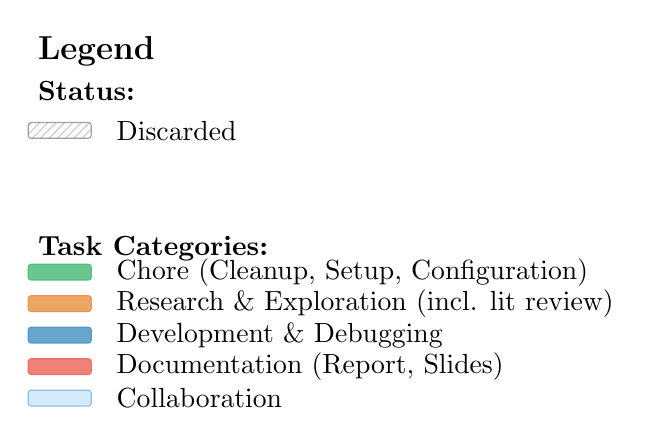
\begin{tikzpicture}
  % Legend title
  \node[anchor=west, font=\bfseries\large] at (0, 4.5) {Legend};

  % Color categories
  \node[anchor=west, font=\bfseries] at (0, 2) {Task Categories:};  % Legend items
  \fill[accentgreen!70, draw=accentgreen!80, rounded corners=1pt] (0, 1.8) rectangle (0.8, 1.6);
  \node[anchor=west] at (1, 1.7) {Chore (Cleanup, Setup, Configuration)};

  \fill[accentorange!70, draw=accentorange!80, rounded corners=1pt] (0, 1.4) rectangle (0.8, 1.2);
  \node[anchor=west] at (1, 1.3) {Research \& Exploration (incl. lit review)};

  \fill[primaryblue!70, draw=primaryblue!80, rounded corners=1pt] (0, 1.0) rectangle (0.8, 0.8);
  \node[anchor=west] at (1, 0.9) {Development \& Debugging};

  \fill[accentred!70, draw=accentred!80, rounded corners=1pt] (0, 0.6) rectangle (0.8, 0.4);
  \node[anchor=west] at (1, 0.5) {Documentation (Report, Slides)};

  \fill[lightblue!50, draw=secondaryblue!60, rounded corners=1pt] (0, 0.2) rectangle (0.8, 0.0);
  \node[anchor=west] at (1, 0.1) {Collaboration};

  % Discarded approaches
  \node[anchor=west, font=\bfseries] at (0, 4) {Status:};
  \fill[discardedgray!50, draw=discardedgray!70, pattern=north east lines, pattern color=discardedgray!40, rounded corners=1pt] (0, 3.6) rectangle (0.8, 3.4);
  \node[anchor=west] at (1, 3.5) {Discarded};

\end{tikzpicture}
\end{document}